\scanpage{42}

automatiquement fermés). \deleted{W.M. prouvent}

Il semble que le théorème suivant soit vrai (dont W.M. prouvent une variante un peu affaiblie) :

a) Si $A_0$ de t.f. sur $k$ est lisse sur $k$, $\exists A$ \inserted{W-M}-Algèbre sur $W$, \uline{plate} sur $W$, et un $k$-isomorphisme
\[
\varphi:A\otimes_W k\simeq A_0.
\]

b) De plus, un tel couple $(A,\varphi)$ est unique à isom (non unique près), i.e. si on a des \deleted{\unsure{cf}} $\overline{\mathrm m}$ $(A',\varphi')$, il existe un $W$-isom $u:A\longrightarrow A'$ rendant comm. le diagramme

\margin{\unsure{faire figure|faire preuve}.}

c) Définissons \inserted{pour tte Algèbre de W.M. $A$ sur $W$,} $\Omega^1(A/W)$ par la propriété universelle pour les dérivations de $A/W$ dans un $A$-module de type fini, d'où
\[
\Omega^*(A/W)=\bigwedge^*(A/W),
\]
qui est un \uline{complexe} de $W$-Algèbres.

\margin{\figure{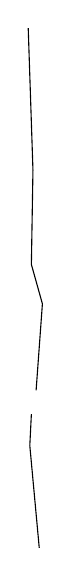
\begin{tikzpicture}
\draw (0,0)--(.06,-1.8)--(.04,-3)--(.18,-3.5)--(.10,-4.6);
\draw (.04,-4.9)--(.02,-5.3)--(.14,-6.6);
\end{tikzpicture}}}

\deleted{\unsure{pour deux} \unsure{soient} \inserted{$A,A'$} $(A,\varphi)$ $(A',\varphi')$ \inserted{et} comme en}

\deleted{b) et \unsure{choisissons} $u:A\overset{\sim}{\longrightarrow}A'$ comme en}

\deleted{\unsure{isom}}

b) $u:A\longrightarrow A'$ un hom de W.M-Algèbres lisses sur $W$, d'où
\diagram{\begin{tikzcd}[ampersand replacement=\&]
u^*:H^i(\Omega^\bullet(A'/W)) \arrow[r,dash] \& H^i(\Omega^*(A'/W))
\end{tikzcd}}

\margin{41}
